%% Template for SDP report, adapted from mlp_cw2_template, 2018. 

%% Based on  LaTeX template for ICML 2017 - example_paper.tex at 
%%  https://2017.icml.cc/Conferences/2017/StyleAuthorInstructions

\documentclass{article}
\usepackage[T1]{fontenc}
\usepackage{amssymb,amsmath}
\usepackage{txfonts}
\usepackage{microtype}
\usepackage{xspace}
\xspaceaddexceptions{\%}

% Lists with less spacing between items
\usepackage{paralist}

% For figures
\usepackage{graphicx}
\usepackage{subfig} 

% For citations
\usepackage{natbib}

% For algorithms
\usepackage{algorithm}
\usepackage{algorithmic}

% the hyperref package is used to produce hyperlinks in the
% resulting PDF.  If this breaks your system, please commend out the
% following usepackage line and replace \usepackage{mlp2017} with
% \usepackage[nohyperref]{mlp2017} below.
\usepackage{hyperref}
\usepackage{url}
\urlstyle{same}

% Packages hyperref and algorithmic misbehave sometimes.  We can fix
% this with the following command.
\newcommand{\theHalgorithm}{\arabic{algorithm}}


% Set up MLP coursework style (based on ICML style)
\usepackage{mlp2018}
\mlptitlerunning{SDP Demo \demoNumber  Group (\groupNumber)}
\bibliographystyle{icml2017}


\DeclareMathOperator{\softmax}{softmax}
\DeclareMathOperator{\sigmoid}{sigmoid}
\DeclareMathOperator{\sgn}{sgn}
\DeclareMathOperator{\relu}{relu}
\DeclareMathOperator{\lrelu}{lrelu}
\DeclareMathOperator{\elu}{elu}
\DeclareMathOperator{\selu}{selu}
\DeclareMathOperator{\maxout}{maxout}







%% You probably do not need to change anything above this comment

%% REPLACE the details in the following commands with your details
\setGroupNumber{10}
\setGroupName{ThreeDots}
\setProductName{Louis}
\setLogoFileName{figs/sdp_logo.png}

\usepackage[table,xcdraw]{xcolor}
% If you use beamer only pass "xcolor=table" option, i.e. \documentclass[xcolor=table]{beamer}
\usepackage[normalem]{ulem}
\useunder{\uline}{\ul}{}

\begin{document} 

\makeSDPTitle{Project Plan}

% Previous MLP Style Title Layout working. 
% \twocolumn[
    % \mlptitle{\productName: SDP Demo \demoNumber}
    % \centerline{Group \groupNumber: \groupName}
% ]

\begin{abstract} 
louis is an affordable, interactive and assistive device for learning braille. It includes an application ecosystem and has a unique, physically-extensible, modular design. First, we will develop a Lego prototype of the main controller and one refreshable character module that can display the letter `A'. We then extend this model to include the full braille character set. Our firmware API will be completed by this point and we will start developing a primary `main' application, as well as a teaching flashcard app. Our next step is to incrementally miniaturize our hardware by replacing parts with smaller, 3D-printed, alternatives. We will develop two additional character modules and showcase our modular design. And finally, we will add audio input support, enabling more advanced apps to be developed and added to the application ecosystem.
\end{abstract}

\section{Goal description} 

Whether it exists on public signage, translated books, or on the back of important medication, braille literacy is an invaluable skill for visually impaired people which gives a freedom in everyday life that sighted people so casually take for granted. Whilst many visually impaired people use braille only for more practical reasons, it is also valuable in a variety of situations, including presenting; Former Home Secretary David Blunkett in 2012 urged people to learn braille saying that even the best computer braille displays and earpieces won't help you do a presentation in the same way as having your information on paper in front of you \cite{braillespreading}.

The problem we are trying to solve is decreasing braille literacy rates among blind or visually impaired people. At a previous estimate fewer than 1\% of visually impaired people in the UK were users of braille \cite{braillespreading}. Our solution is an interactive refreshable braille robot, coupled with fun and approachable software which can help both children and adults learn the universally accepted and useful system of braille. 

\subsection{Relevance of the system} 

Since louis primarily serves as an aid to learn and interact with braille, our product will be most relevant to visually impaired people and their support network (parents, teachers, etc.).

\subsubsection{The importance of braille}

It has been argued that braille is becoming a less relevant tool, given digital technologies prevalence throughout our society. However, studies have shown that students who can read braille tend to acquire higher literacy rates \cite{earlybraille}. And a survey conducted by Louisiana Tech University found that people who learn braille have a much higher chance of securing a job \cite{transformingbraille}. Braille education is crucial to literacy, and literacy is crucial to employment.

louis also allows users to learn skills such as spelling, punctuation and capitalisation, whereas the alternative, audio, does not. Audiobooks have provided an excellent additional resource for reading comprehension, but passive listening does not have the same effect as active reading and writing. Audio transcription is also not always appropriate or viable in certain situations, for example in a crowded lift. Braille offers a system for labelling all kinds of items (like lift buttons and medicines) which aids independence and raises self-esteem.

\subsubsection{The current market}

Even though learning braille has been proven to be beneficial, literacy rates are low. In the UK less than 5\% of legally blind people have the ability to read braille \cite{brailleprofiling}. Among the causes are school budget constraints and personal financial limitations. The prices of the current devices on the market are described by users as ``\emph{phenomenally high}'' \cite{brailledisplays}, and justly so. Modern notetakers, which include some Android and Windows applications, are sold for more than \pounds 800 and learning tools are priced at over \$2,000. Another issue raised in the user research is the necessary repairs, which are ``\emph{extremely inconvenient, [...] not to mention the expense}'' \cite{brailledisplays}. Our modular architecture of the display means that users won't have to go without their devices, as they will be able to use as many, or as few, braille cells as they need. This also keeps the initial cost of our product low, with `pay-for-what-you-use' characters to grow your braille display.

Moreover, most refreshable braille learning devices that are currently on the market are aimed at children, whereas our product is aimed at users of all ages. It can support all kinds of learning apps, as well as serve as a more general assistant. With our open SDK, our robot can be useful, relevant and accessible to everyone.


\subsection{High-level description} 

louis is primarily a voice controlled learning assistant, complete with a speaker, that helps visually impaired individuals learn braille easily and conveniently. It makes use of quizzes and games to allow its users to learn from basic braille characters to more advanced concepts such as contractions.

A unique aspect of louis that distinguishes itself from its competitors is that it has a modular architecture for both software and hardware, therefore the users only need to purchase as many parts as they believe will be helpful. This would give an affordable opportunity for any of those people wanting to learn braille, but are unable to do so due to the current financial boundaries. louis also provides an application ecosystem where developers can build software using the development toolkit included with the product. Developers could create new tools and applications such as an app to read news headlines, an Alexa integration, a braille music tutor and countless others. The open approach with software development makes our product truly useful beyond our small team.

\subsubsection{User Stories}

\begin{enumerate}
  \item As a user, I can learn braille by using a flashcard app on the device.
  \item As a user with a limited budget, I find louis a lot more affordable than its competitors as I only need to purchase parts that I believe will be useful.
  \item As a visually impaired user, I can open applications of my choice with my voice.
  \item As a developer, I can build applications on the platform louis provides using the given development toolkit.
\end{enumerate}

\section{Task planning}

We have identified our main technical goals to be the following: 
\begin{enumerate}
  \item User selection of letters display speed and application
  \item Start of flashcard or other application
  \item Choice of next letters to display by application 
  \item Output of braille letters on device cells 
  \item Output of letters on speakers 
\end{enumerate}

The two main dependencies concern the output of braille letters, as the teaching purpose of the device entirely depends on the braille representation to also be translated and repeated out loud to the user. 
 
Another one concerns user input, in terms of application selection and letter display speeds. The input method can be chosen at a later date, as physical or audio inputs would yield the same results, but this information needs to be present first before the device can generate the next letters for display. 
 
These main system requirements are summarized in the goal model shown in Figure \ref{fig:goalmodel}.

\begin{figure*}[h]
\vskip 5mm
\begin{center}
\centerline{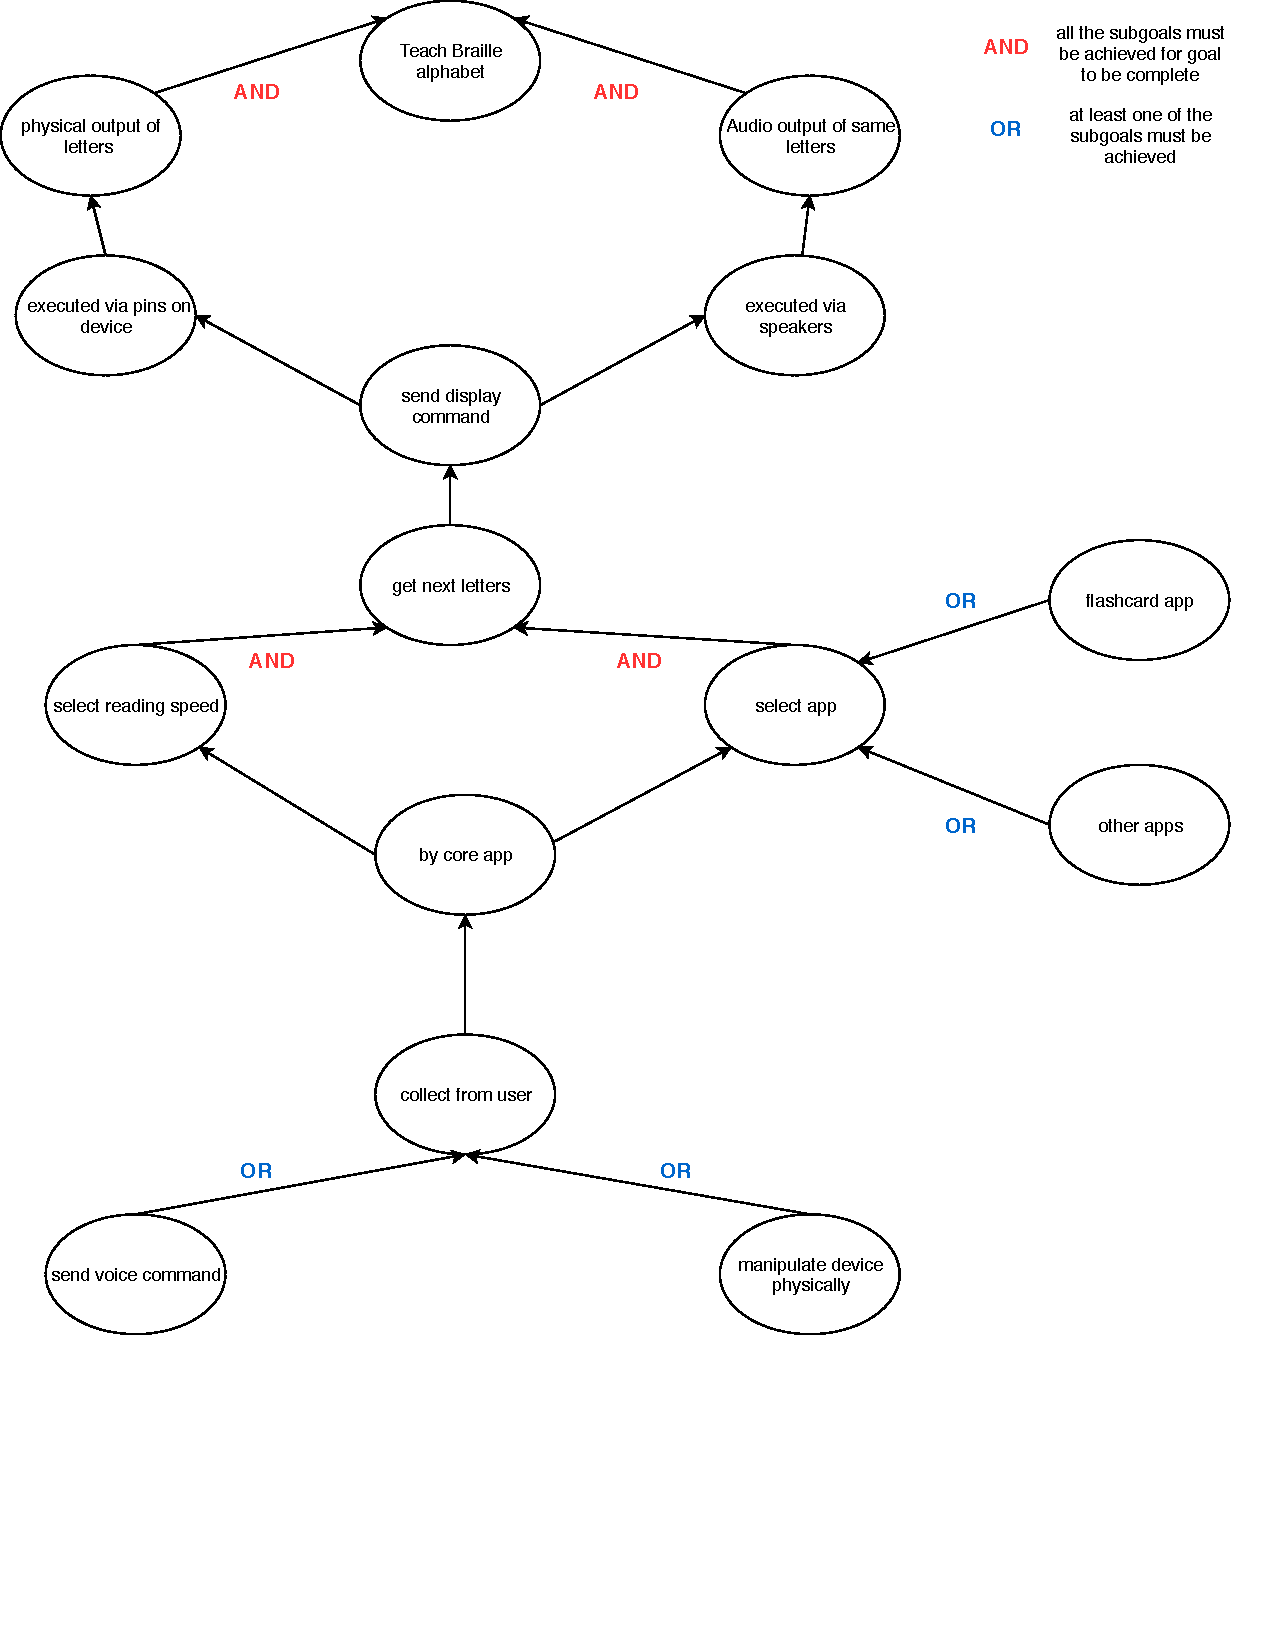
\includegraphics[width=\textwidth]{figs/goalmodeling}}
\caption{System Requirements Goal Model}
\label{fig:goalmodel}
\end{center}
\vskip -5mm
\end{figure*} 

\subsection{Milestones} 

We have defined the following milestones and evaluation methods based on the technical goals defined in the section above:

\subsubsection{Hardware}

\begin{enumerate}
  \item Working display mechanism with pins
  \begin{enumerate}
    \item Milestones:
    \begin{enumerate}
      \item Motor rotates, pins move up and down
      \item Two additional 3D-printed cells
      \item Audio or physical input integration: user passes on selections
    \end{enumerate}
    \item Evidence and evaluation:
    \begin{enumerate}
      \item Correct display of one specific letter (e.g `A')
      \item Correct display of sequence of three letters
      \item Audio output confirming speed and app choice
    \end{enumerate}
  \end{enumerate}
  \item Casing
  \begin{enumerate}
    \item Milestones:
    \begin{enumerate}
      \item Prototype in Lego
      \item 3D-printed prototype
      \item Enclosure and fittings
    \end{enumerate}
  \end{enumerate}
\end{enumerate}

\subsubsection{Firmware and Software}

\begin{enumerate}
  \item Milestones:
  \begin{enumerate}
    \item Core app passes on hardcoded letter to display
    \item Physical and audio output of letters and Flashcard app: core app passes on flashcard app letters at given speed
    \item App selection and reading speed selection: core app receives either audio or physical selection from user for display speed and app
    \item Other app(s): core app receives user app choice and selects correct one
  \end{enumerate}
  \item Evidence and evaluation:
  \begin{enumerate}
    \item Letter displayed after a reasonable amount of time
    \item Physical and audio display of letters at correctly timed intervals (and audio output returned after physical, also timed appropriately (tbd))
    \item Letters displayed at correct speed for each choice (can time it); correct app selected
    \item Correct letter sequence for each additional app is returned
    \begin{enumerate}
      \item Motor rotates, pins move up and down
      \item Two additional 3D-printed cells
      \item Audio or physical input integration: user passes on selections
    \end{enumerate}
    \item Evidence and evaluation:
    \begin{enumerate}
      \item Correct display of one specific letter (e.g `A')
      \item Correct display of sequence of three letters
      \item Audio output confirming speed and app choice
    \end{enumerate}
  \end{enumerate}
\end{enumerate}


\subsection{Task decomposition}

The required tasks for the project were split into atomic units. A Gantt chart, shown in Figure \ref{fig:gantt}, shows the progression of these atomic units throught the time available for the task, as well as highlighting the dependencies between the atomic units.

\begin{figure*}[h]
\vskip 5mm
\begin{center}
\centerline{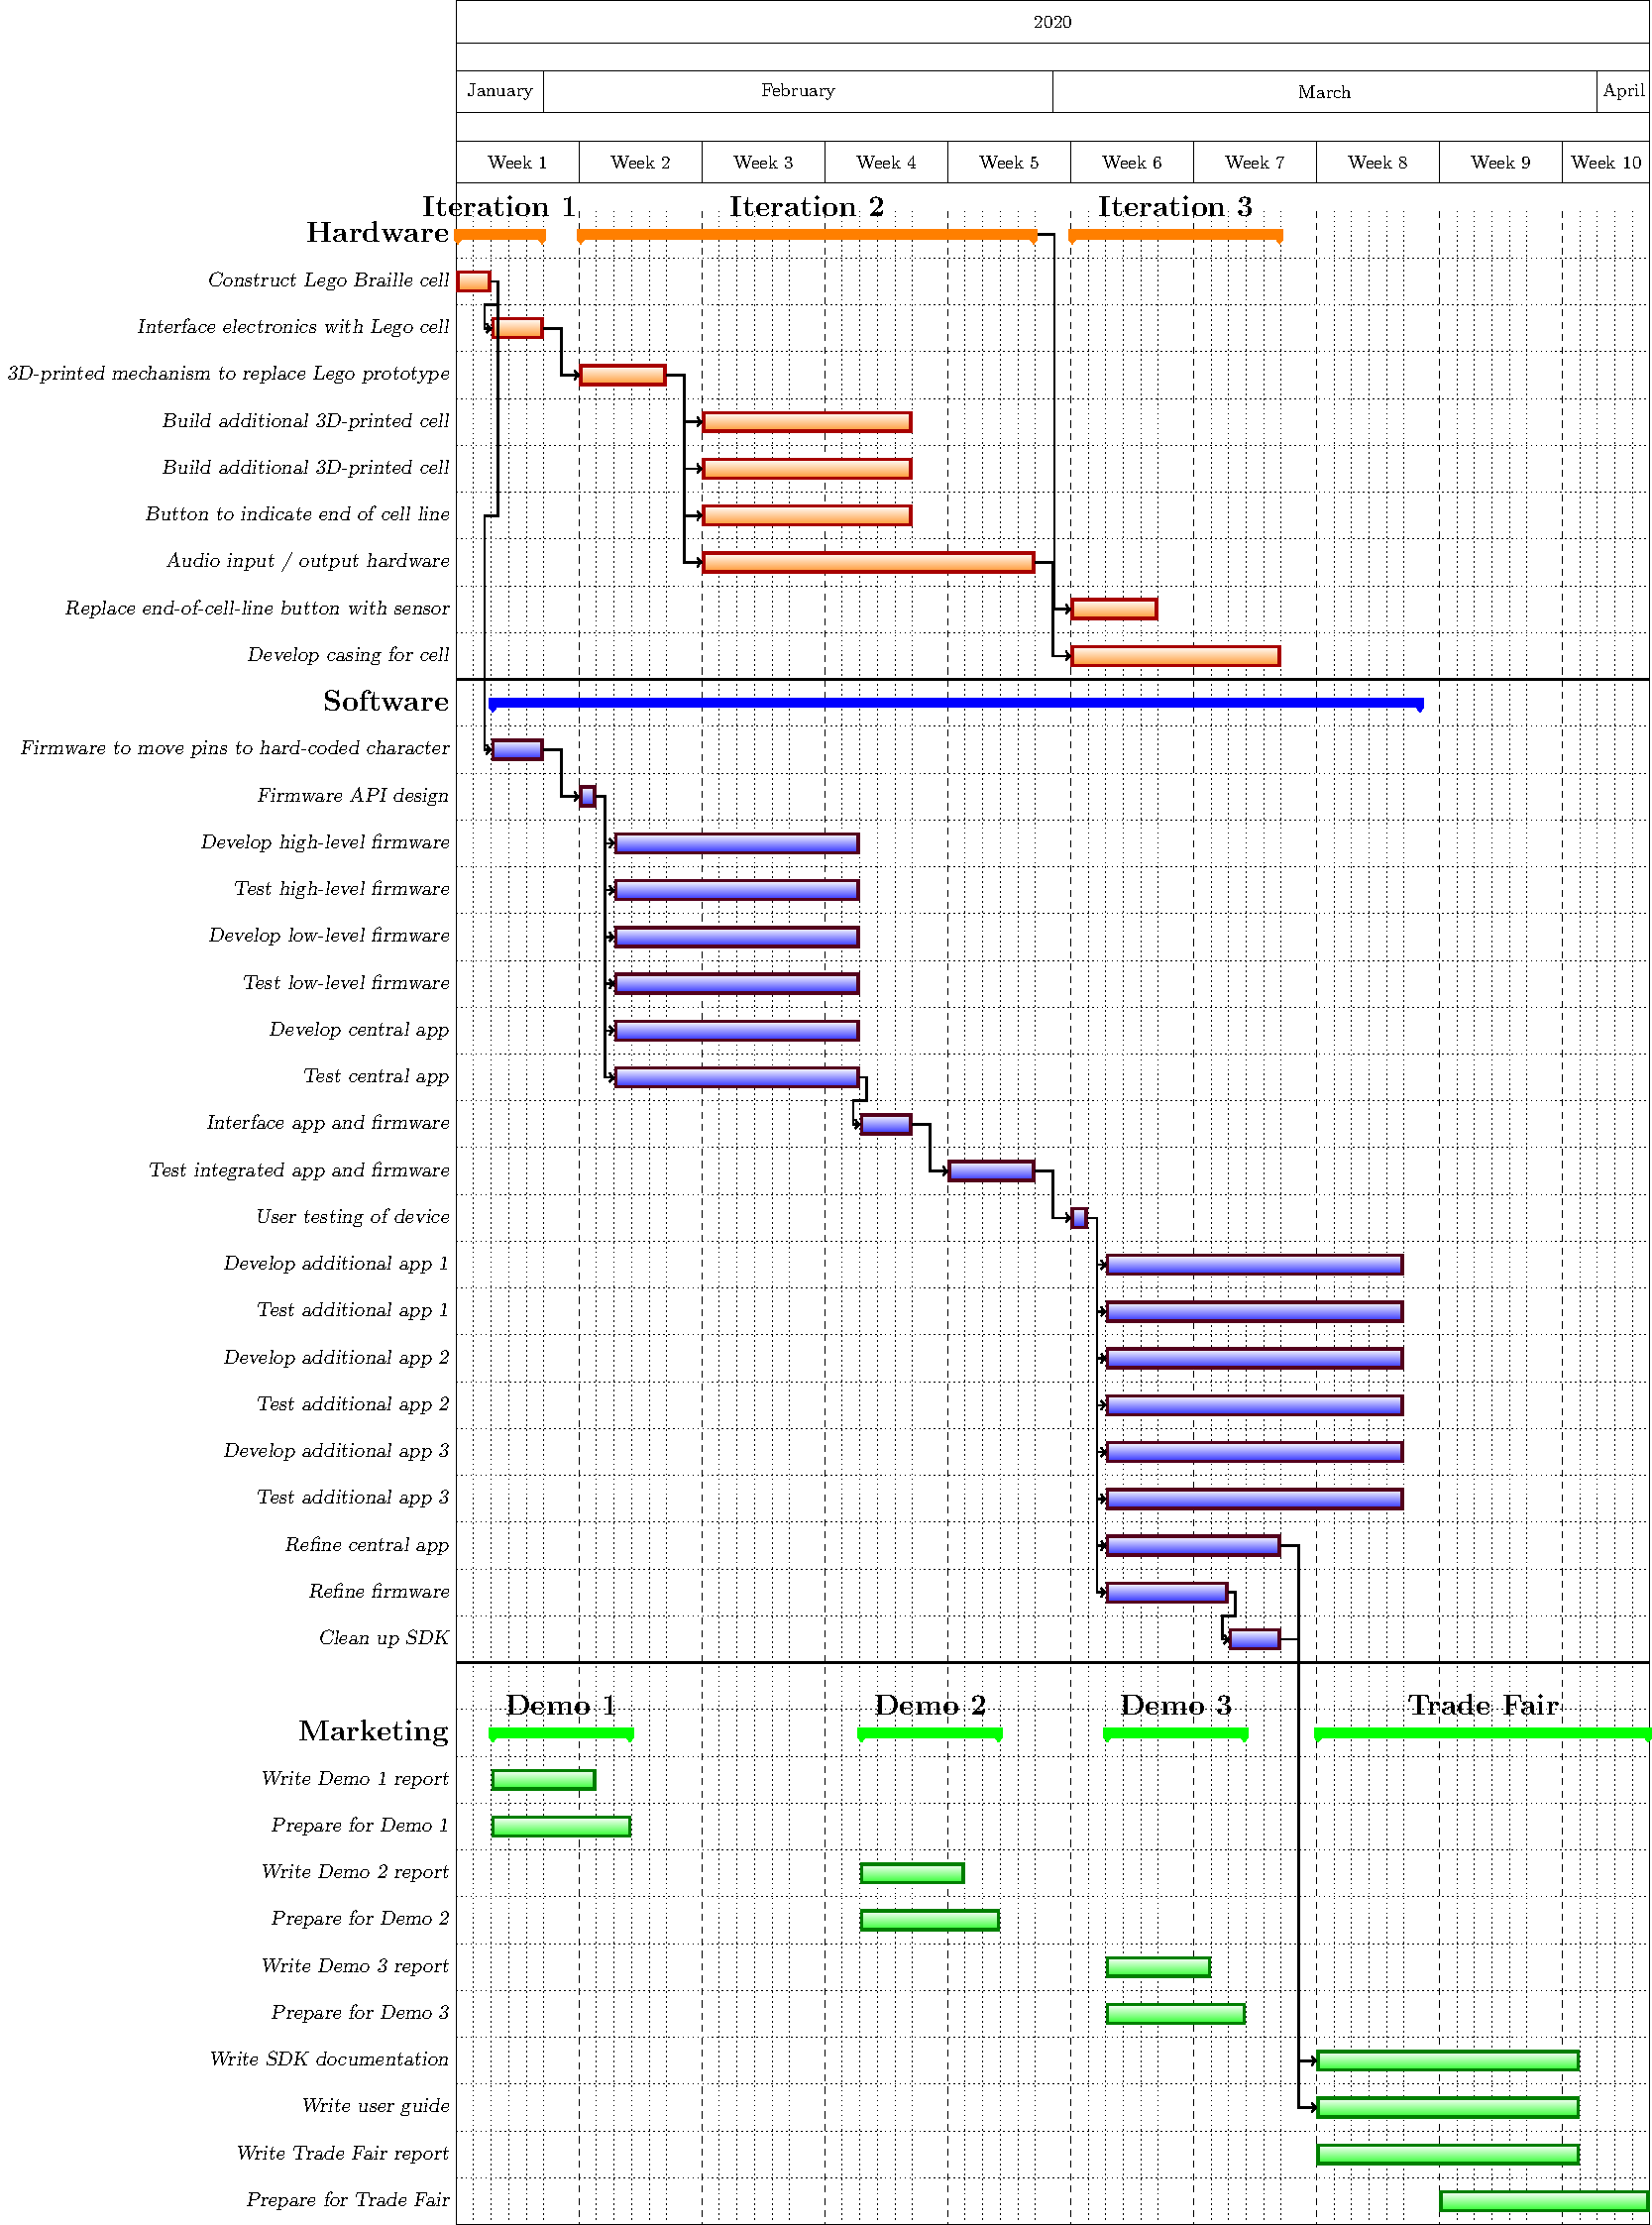
\includegraphics[height=\textheight]{figs/gantttest}}
\caption{Gantt chart of task decomposition and dependencies}
\label{fig:gantt}
\end{center}
\vskip -5mm
\end{figure*} 

To make the high-level tasks more manageable, we will be routinely incorporating story decomposition into our workflow. The process comes from the agile methodology, as outlined in the workshop for project planning. By breaking down stories into smaller tasks, we hope to increase iteration speeds and regularly deliver incremental value gains.


\subsection{Resource distribution}

\subsubsection{Human resources}

Our company, ThreeDots, is composed of ten members. Over the next 11 weeks, each will commit approximately 200 hours to our project, louis.

Ten percent of this time will be remitted to allow individuals to complete their final report. This is proportional to the allocated marks (relative to the rest of the project), as well as to the time available after the final demonstration (one week).

This leaves 180 hours per capita, (a combined 1,800 hours), to allocate between:
\begin{enumerate}
  \item Iterating on hardware, firmware and software
  \item Preparing for, and presenting at, demonstrations and workshops
  \item Creating reports, user guides and other technical documentation
  \item Administrating and participating in meetings
  \item Performing market research and product evaluation
\end{enumerate}

The allocation of these hours is shown in Table \ref{table:hours}.

\begin{table}[]
\begin{center}
\begin{small}
\begin{tabular}{|l|l|}
\hline
\rowcolor[HTML]{C0C0C0} 
Task                           & Hours \\ \hline
Hardware                       &       \\
\quad First iteration                & 87    \\
\quad Second iteration               & 116   \\
\quad Third iteration                & 87    \\
\quad Enclosure and fittings         & 95    \\ \hline
Firmware \& Software           &       \\
\quad Firmware                       & 90    \\
\quad Central application            & 141   \\
\quad Additional applications        & 345   \\ \hline
First demonstration            &       \\
\quad Report                         & 40    \\
\quad Meeting                        & 10    \\ \hline
Second demonstration           &       \\
\quad Report                         & 40    \\
\quad Meeting                        & 10    \\ \hline
Third demonstration            &       \\
\quad Report                         & 36    \\
\quad Meeting                        & 10    \\
\quad User Guide                     & 60    \\ \hline
Trade Fair                     &       \\
\quad Report                         & 50    \\
\quad Meeting                        & 80    \\ \hline
Support                        &       \\
\quad Workshops                      & 20    \\
\quad Q\&A sessions and office hours & 20    \\ \hline
Meetings                       &       \\
\quad Scheduled (with mentor)        & 120   \\
\quad Additional (impromptu)         & 140   \\ \hline
Market Research                &       \\
\quad Ethics                         & 8     \\
\quad Initial contact                & 5     \\
\quad First session                  & 5     \\
\quad Second session                 & 5     \\ \hline
Total                          & 1620  \\ \hline
\end{tabular}
\end{small}
\caption{Human Resource Allocation}
\label{table:hours}
\end{center}
\end{table}

Intentionally, we have failed to assign 10 percent of the available time, to account for natural project slippage and alleviate unforeseen delays.

\subsubsection{Hardware, Finance and Technician Time Budgeting}

Initially, we will create a proof-of-concept hardware design using the Lego EV3 Mindstorms kits that have been provided, and incrementally replace various parts with 3D-printed pieces. This will allow us to miniaturize our components, and create custom structures. We also plan to utilize the Raspberry Pi micro-computer to act as the main robot controller, and to interface with the audio I/O.

Financial budgeting and the tracking of technician time will be completed using a shared Google Sheets file to ensure transparency within the group, and allow for adequate planning. We anticipate that the majority of both resources will be consumed by 3D-printing these custom parts to miniaturize our hardware. Finally, we hope to enclose our components in a branded acrylic plastic enclosure to help with marketing the robot. To minimize inflicted costs, we will utilize some group members' previous personal experience to create CAD designs, and export to STL models for printing, engraving etc.

At this time, we do not anticipate requiring any custom, externally-ordered components.

The simplified bill of materials and budget estimation calculations have been provided in Table \ref{table:budget}.

\begin{table}[]
\begin{center}
\begin{small}
\begin{tabular}{|p{3cm}|p{1.5cm}|p{1.5cm}|}
\hline
\rowcolor[HTML]{C0C0C0} 
Item                    & Technician Cost (hours) & Financial Cost (\pounds) \\ \hline
Lego EV3 Mindstorms Kit & -                       & -                  \\ \hline
Raspberry Pi            & -                       & -                  \\ \hline
3D-printed Components   & 4.5                     & 40                 \\ \hline
Wiring                  & -                       & 8                  \\ \hline
Acrylic enclosure       & 4                       & 30                 \\ \hline
Miscellaneous           & 1.5                     & 20                 \\ \hline
Total Cost              & 10                      & 98                 \\ \hline
\end{tabular}
\end{small}
\end{center}
\caption{Simplified Bill of Materials and Budget Estimation}
\label{table:budget}
\end{table}

\subsection{Risk assessment}

Risks regarding the project and its development were measured with respect to Table \ref{table:severity} and Table \ref{table:likelihood}.

\begin{table}[h]
\begin{center}
\begin{small}
\begin{tabular}{|l|p{3cm}|}
\hline
\rowcolor[HTML]{C0C0C0}Scale of Risk & Severity of Risk                        \\ \hline
Low (1)    & Little to no impact                                               \\ \hline
Medium (2) & Would affect the progress of the project, but it can be contained \\ \hline
High (3)   & Major setback                                                     \\ \hline
\end{tabular}
\end{small}
\end{center}
\caption{Severity of Risk}
\label{table:severity}
\end{table}

\begin{table}[h]
\begin{center}
\begin{small}
\begin{tabular}{|l|p{3cm}|}
\hline
\rowcolor[HTML]{C0C0C0}Scale of Risk & Likelihood of Risk                     \\ \hline
Low (1)    & Unlikely, but possible                                            \\ \hline
Medium (2) & May occur, but not very likely                                    \\ \hline
High (3)   & Risk is likely to occur                                           \\ \hline
\end{tabular}
\end{small}
\end{center}
\caption{Likelihood of Risk}
\label{table:likelihood}
\end{table}

Potential risks identified and corresponding actions that will be taken if we are required to face them are described in Table \ref{table:riskstable}.

\begin{table*}[h]
\begin{center}
\begin{small}
\begin{tabular}{|p{3cm}|p{3cm}|p{3cm}|p{0.5cm}|p{0.5cm}|p{3cm}|}
\hline
\rowcolor[HTML]{C0C0C0} 
Risk                                                                                              & Impact on project                                                                                               & Measures taken to minimize                                                                                                                                                                                & Severity & Likelihood & Contingency plan                                                                                                                                  \\ \hline
Incorrect translation to Braille from alphabet                                                    & Device works fine, but becomes not usable                                                                       & We will be studying the direct translation and making sure that each letter is translated correctly                                                                                                       & 3        & 1          & Allow for testing time, to check that machine works as intended                                                                                   \\ \hline
Team member becomes unavailable due to emergency and/or absence                                   & Work falls off schedule or is submitted but incomplete                                                          & Multiple group members are assigned to each team, so that work is divided and easily taken over if needed                                                                                                 & 3        & 2          & Team members with less workload should switch teams if needed                                                                                     \\ \hline
Hardware falls apart                                                                              & Device is not able to work. Will lose time on fixing and retesting the device                                   & Allocated 10\% of our resources in time and budget for potential mishaps and this is included                                                                                                             & 3        & 2          & Finish with the hardware as early as possible, so that to allow for any problems to be spotted as well as avoid any last minute risk              \\ \hline
Clashes between team members ideas/working hours/working styles                                   & Lose communication between members, team is not focused on tasks and there could be delays into completing them & Ideas are run through the team and are evaluated in terms of feasibility and effectiveness. Times and style are discussed between team members from the beginning and are followed so as to avoid clashes & 3        & 2          & If a clash is not resolved within the team, then the issue is raised in the entirety of the group and if needed to the Course Organisers          \\ \hline
Device is not easy to use                                                                         & The purpose of the machine is defeated, since most of the users will not be able to use it                      & Research project and produce a good System Design. Be in cooperation with a visually impared person suitable to establish if the device is hard to use. Establish modularity of the design                & 3        & 1          & Allocate testing time to allow for adjustments to be made easily. If it cannot be completely simple, then maybe rethink the purpose of the device \\ \hline
Delays in building functional hardware results in delays in building the software.                & Might result in producing an incomplete application with regards to software                                    & Once the first prototype of the braille cell mechanism is built, software and hardware development can be done in parallel                                                                                & 3        & 1          & Allocated 10\% of our time in potential delays and errors                                                                                         \\ \hline
Problem in building the original prototype of the braille cell mechanism entirely from lego parts & Delays in building the hardware, as it is the main aim for the first demo                                       & Design the system in detail and adapt to any adjustments needed as an initial compromise and improve in 2nd iteration                                                                                     & 3        & 1          & 3D print the required parts and complete the lego structure                                                                                       \\ \hline
Not able to create each braille cell as small as possible                                         & Device is considerably bigger than initially estimated and thus more material is used; bigger budget            & Thorough system design including hardware and software, as well as budget allocation                                                                                                                      & 3        & 1          & Adjust our goal, so that we are more flexible regarding the size of the cell                                                                      \\ \hline
Not successful in creating several quizzes and games                                              & Some of the purposes of the device are not developed                                                            & Ensure we build applications that are easy; correct study and design of software                                                                                                                          & 3        & 2          & Adjust our goal; maybe focus on building one game to present as a prototype                                                                       \\ \hline
\end{tabular}
\end{small}
\end{center}
\caption{Identified risks and corresponding actions}
\label{table:riskstable}
\end{table*}

\subsubsection{Strengths, weaknesses, opportunities and threats}

The strengths, weaknesses, opportunities and threats of this project have been outlined in Table \ref{table:swottable}.

\begin{table*}[h]
\begin{center}
\begin{tabular}{|p{8cm}|p{8cm}|}
\hline
\rowcolor[HTML]{C0C0C0} 
Strengths (internal factors)                                                                                                                                                                                                                                      & Weaknesses (internal factors)                                                                                          \\ \hline
\begin{enumerate}
  \item Experience and Skill levels (hardware designing, low and high-level programming, and marketing)
  \item Resource availability (Lego, controllers, and 3D printer)
  \item Unique solution - no other product alike on market.
  \item Effective leadership and planning
  \item Clearly defined goals
\end{enumerate} & \begin{enumerate}
  \item Gaps in knowledge and expertise
  \item Unforeseen technical challenges(both software and hardware)
  \item Other members' commitments
\end{enumerate} \\ \hline
\rowcolor[HTML]{C0C0C0} 
Opportunities (external factors)                                                                                                                                                                                                                                  & Threats (external factors)                                                                                             \\ \hline
\begin{enumerate}
  \item Technology and infrastructure development
  \item Market demand
  \item Availability of potential testers of our product
\end{enumerate}                                                                                                                                                            & \begin{enumerate}
  \item Timescale and deadlines
  \item Other competitors' solutions on market
  \item Limited budget
\end{enumerate}                                            \\ \hline
\end{tabular}
\end{center}
\caption{Strengths, weaknesses, opportunites and risks}
\label{table:swottable}
\end{table*}

\section{Group organisation}

The organisational structure is based on the distribution of pre-existing skills as to increase the probability of on-time delivery of the project while still accommodating individual team members' desire to learn new skills in areas they lack expertise. The project manager is mainly responsible for activity and resource allocation, as well as risk analysis and contingency planning, whereas the secretary is mainly concerned with the management of deadlines and meeting planning.

The rest of the team is divided into the functional units of \it{hardware} and \it{software}, and sub-units for system design, and low-level/high-level for software. Communication between the system design role of hardware and software is essential in order to ensure the interoperability of the systems developed independently by the team members.

All communication is handled on Slack to avoid scattering of information and to ensure consistency and transparency. The number of channels is reduced to a minimum.

Fixed weekly meetings for the whole team are scheduled in advance to ensure the availability of all team members to discuss the current progress of the project and potentially plan adjustment measures. Additionally, team members are committed to daily stand-ups on Slack with the aim of synchronizing information among the team and identifying potential issues.

Code-sharing and version control are all handled using git and GitHub. In order to guarantee the cleanliness and functionality of the code base, a contribution procedure is enforced by which commits cannot be pushed directly to the master branch but must be submitted using pull requests. The pull requests are then peer-reviewed by other team members and automatically checked for compilation errors in the continuous integration pipeline.

A graph detailing the group subdivision by functional unit is included in Figure \ref{fig:organisation}.

\begin{figure*}[h]
\vskip 5mm
\begin{center}
\centerline{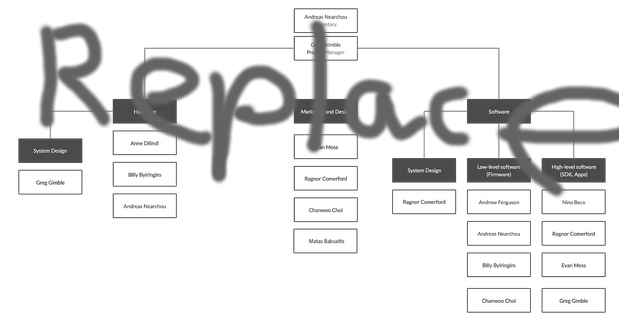
\includegraphics[width=\textwidth]{figs/organisation}}
\caption{Group member organisation and subdivision by functional unit}
\label{fig:organisation}
\end{center}
\vskip -5mm
\end{figure*} 

\bibliography{example-refs}

\end{document} 
